% !TEX program = xelatex
\documentclass[12pt]{article}
\usepackage[margin=1in]{geometry}
\usepackage{nopageno} % no page numbers
\usepackage{setspace} \doublespacing

\usepackage{graphicx}
\graphicspath{ {./graphics/} }
\usepackage[dvipsnames]{xcolor}
\definecolor{CrispBlue}{HTML}{0176AE}

\usepackage{fontspec}
\usepackage{tcolorbox}
\usepackage{etoolbox}
\BeforeBeginEnvironment{verbatim*}{\begin{tcolorbox}[colback=CrispBlue!5!white,colframe=CrispBlue!75!black]}%
\AfterEndEnvironment{verbatim*}{\end{tcolorbox}}%

\usepackage{hyperref}
\hypersetup{
    colorlinks,
    citecolor=black,
    filecolor=black,
    linkcolor=black,
    urlcolor=black
}

\renewcommand{\footnotesize}{\fontsize{8pt}{10pt}\selectfont}


\usepackage[labelfont={small,sc,bf},textfont={small,sc,bf}]{caption}
\setlength{\parindent}{24pt}
% \setlength{\parskip}{1em}

\usepackage{tocloft}
\renewcommand{\cftpartleader}{\cftdotfill{\cftdotsep}}
\renewcommand{\cftsecleader}{\cftdotfill{\cftdotsep}}

\usepackage[shortlabels]{enumitem}

\usepackage{lastpage}
\usepackage{fancyhdr}
\pagestyle{fancy}
\fancyhf{}
\renewcommand{\headrulewidth}{0pt}
\rfoot{Page \thepage\ of \pageref*{LastPage}}

\usepackage{amsmath,amsfonts,amssymb}
\usepackage{bm}
\usepackage{mathtools}

\renewcommand{\listfigurename}{List of Figures}

\begin{document}
\setmainfont{SF Pro Text}
\setsansfont{SF Pro Text}
\setmonofont{SF Mono}
\renewcommand{\familydefault}{\sfdefault}

\hypersetup{
    linkcolor=CrispBlue,
    urlcolor=CrispBlue,
    breaklinks=true
}

\noindent David Kirby\\
ECE 595: Advanced Technical Cybersecurity\\
Spring, 2022
\begin{center}
    \large\bfseries Capture the Flag
\end{center}

The first part of this three-part reverse-engineering exercise was to determine the function name using the nm or readelf commands (see Figure~\ref{fig:readelf}). The next part was to take a look at the disassembled code in GDB (with the pwndbg interface) to determine the purpose of the function (see Figure~\ref{fig:disas}). We can see that the assembly code uses two C library functions -- \texttt{snprint} and \texttt{strncat}, along with a series of jumps and moves. If we compare this to the disassembled code of our previous assignment, we see that the use of jumps and moves is similar to the ones we saw in our for and while loops. This lead me to believe that we were dealing with a loop function. It turns out that running through our \texttt{main} function, and setting breakpoints at the called functions, we see that the program is performing an iterative loop that multiplies i by i and prints the result. It goes through this iteration five times, with the result of each iteration then concatenated with the string \texttt{\_msg} as shown below. The final contents of the buffer at program termination are \texttt{16\_msg}.

\begin{tcolorbox}[colback=CrispBlue!5!white,colframe=CrispBlue!75!black,title=Output of five iterations of the function.]\setstretch{1.25}
0\\
0\_msg\\
1\\
1\_msg\\
4\\
4\_msg\\
9\\
9\_msg\\
16\\
16\_msg
\end{tcolorbox}

\begin{figure}[!ht]
    \centering
    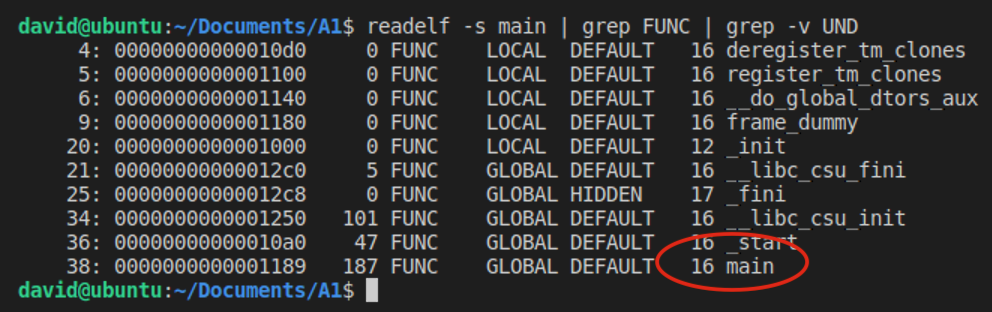
\includegraphics[width=0.81\textwidth]{figure05.png}
    \caption{Determining the function name using \texttt{readelf}.}
    \label{fig:readelf}
\end{figure}

\begin{figure}[!ht]
    \centering
    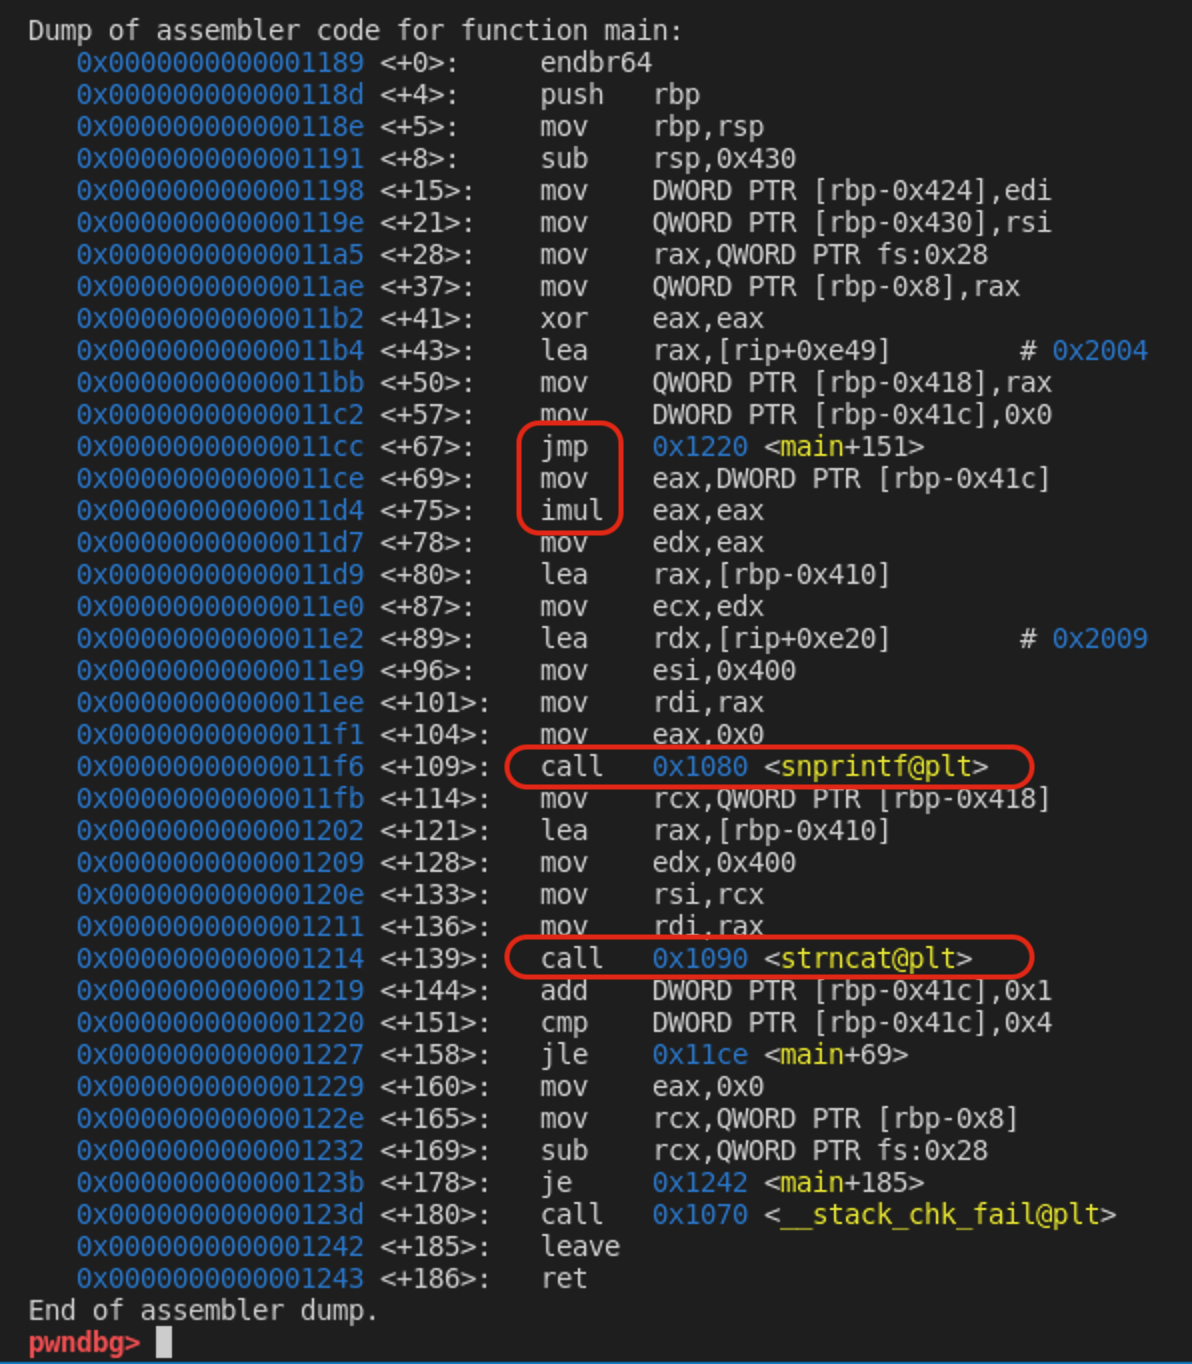
\includegraphics[width=0.82\textwidth]{figure06.png}
    \caption{Disassembled code using \texttt{GDB}.}
    \label{fig:disas}
\end{figure}

\begin{figure}[!ht]
    \centering
    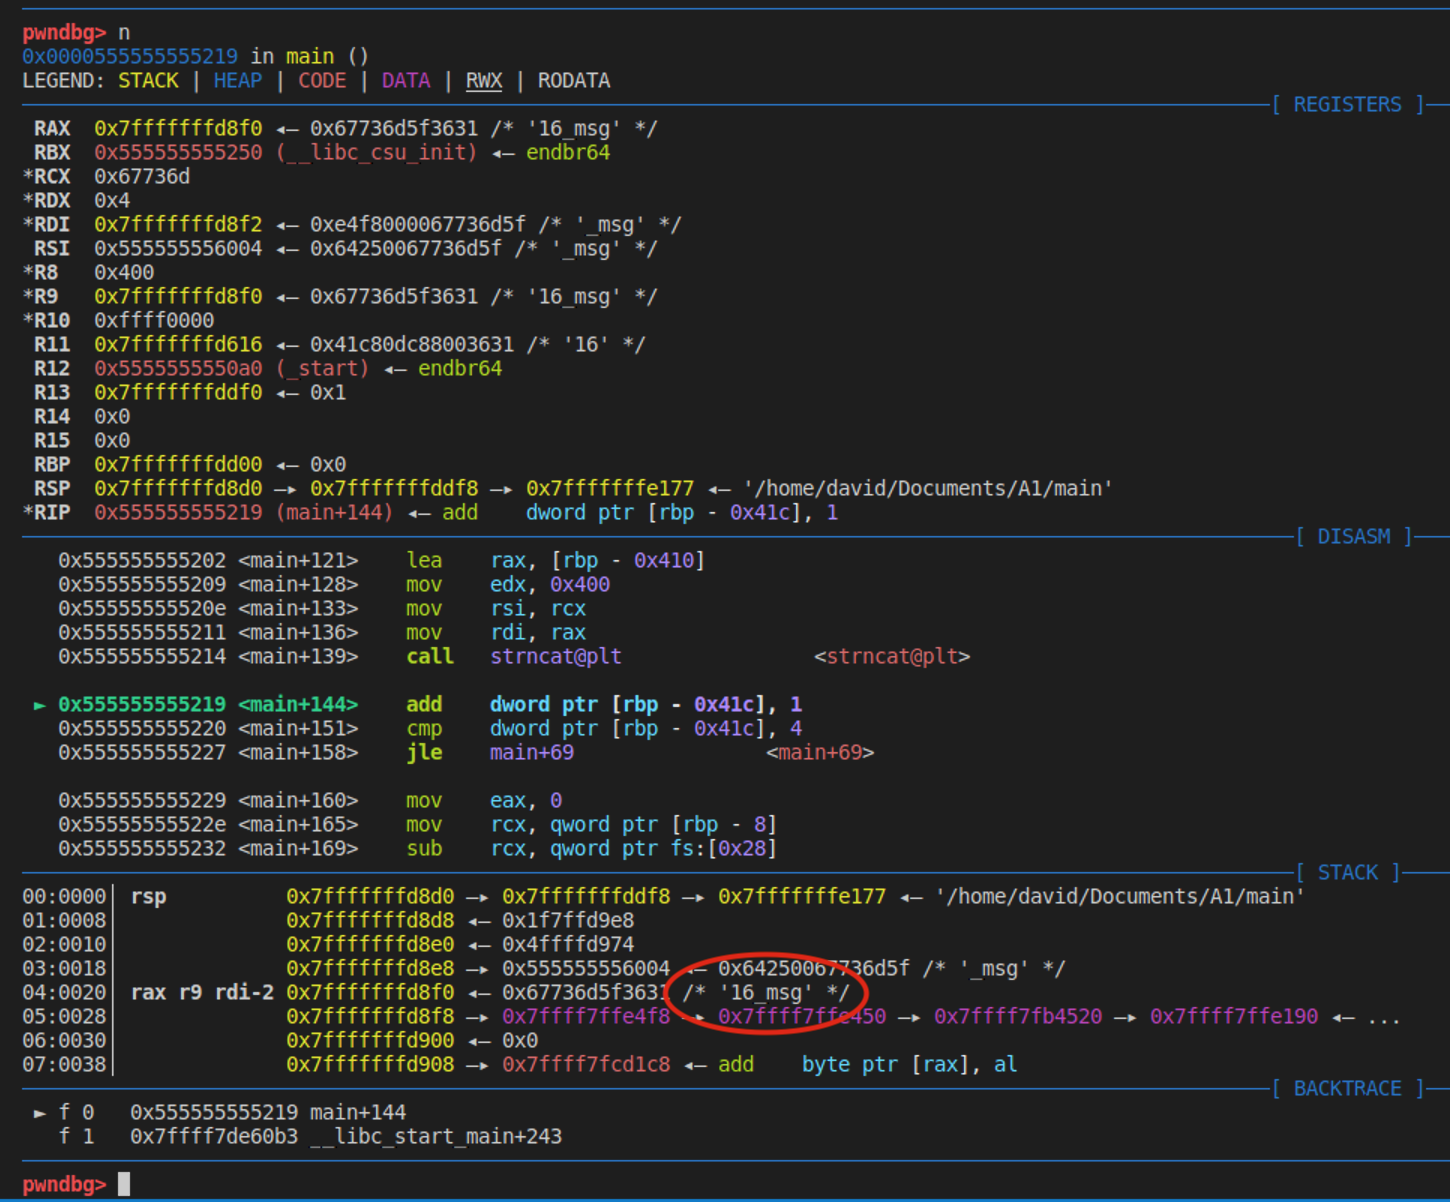
\includegraphics[width=\textwidth]{figure07.png}
    \caption{Stack showing concatenated message.}
    \label{fig:stack}
\end{figure}

\end{document}